\documentclass[journal]{IEEEtran}
\usepackage[T1]{fontenc}
\usepackage[utf8]{inputenc}
\usepackage{amsmath,amssymb,booktabs,array,graphicx,url,cite}
\usepackage[hidelinks]{hyperref}
\usepackage{placeins,balance}
\graphicspath{{../results/figures/}}
\newcommand{\R}{\mathbb{R}}
\hyphenation{LightGBM SARIMAX}
\begin{document}
\title{Dynamic Pricing and Demand Forecasting for Sports Facility Aggregators}
\author{Kuandyk Bibarys and Tulebay Aslan\\Astana IT University, Astana, Kazakhstan}
\maketitle
\begin{abstract}
This study evaluates a forecasting and pricing pipeline for bookable sports facilities using a reproducible synthetic dataset. The data contain 153,300 hourly slots across 14 simulated venues over 730 days. Chronological validation selects a forecasting model, and the final 146 days are held out for evaluation. Logistic regression, LightGBM, an LSTM and a SARIMAX baseline are compared with historical booking climatology. A separately estimated price-response layer supports constrained profit optimization. Revenue, utilization and cancellations are evaluated under common counterfactual assumptions and checked against the simulator's known mechanism. All results are preliminary simulation measurements. They do not establish real-world price elasticity, customer behaviour or commercial performance.
\end{abstract}
\begin{IEEEkeywords}
dynamic pricing, demand forecasting, sports facilities, synthetic data, simulation, booking probability
\end{IEEEkeywords}
\section{Introduction}
Sports facility aggregators sell capacity that expires. An empty court or pitch cannot recover the revenue from a slot once its start time has passed. Demand varies with time, weather, facility type and price. The research problem is how to forecast booking probability and use that forecast to choose prices within constraints set by facility owners.

The literature review and original Methods proposed an integrated forecasting and pricing study using real aggregator records. The present article reports a preliminary simulation using the supplied booking generator. The simulated records permit evaluation of forecasts and pricing calculations against a known booking mechanism. They do not provide evidence about the behaviour of actual customers or the revenue of an operating aggregator.

The review asked which forecasting methods and external variables are useful, how pricing research represents price response and capacity, and which gaps remain for bookable sports facilities. These questions lead to three operational questions for the experiment. RQ1 asks whether the selected forecasting model improves probabilistic accuracy over the baselines. RQ2 asks what revenue change the constrained pricing policy produces in the simulation, including its uncertainty and agreement with the simulator. RQ3 asks whether that policy increases weekday off-peak occupancy without an unacceptable increase in cancellations. The success criteria proposed in Methods are retained, subject to the deviations stated below.

\section{Literature review}
The supplied review contains 13 original studies and 10 review papers published from 2021 to 2025. Its search covered scholarly journal sources and publisher or institutional records from ScienceDirect, Springer Nature, INFORMS, Wiley, ACM, MDPI and related indexes. The selection excluded conference proceedings, book chapters and unpublished preprints. The methodological references added in the Methods section serve a different purpose and are not counted as part of this review corpus.


\subsection{Pricing and marketplace mechanisms}

\subsubsection{Surge pricing and two-sided temporal responses}
Hu, Hu, and Zhu study surge pricing in ride-hailing marketplaces and focus on the fact that riders and drivers respond to prices at different speeds \cite{r2}. The problem is therefore not simply choosing a price but understanding the temporal interaction between two sides of a platform. Their methodology uses a two-period game-theoretic model with strategic consumer and driver responses. The study identifies shortlived high-price ``skimming'' surge and low-initial/high-later ``penetration'' surge equilibria, with the latter depending on information sharing with drivers. The contribution is a formal demonstration that the timing of behavioral responses changes the performance of dynamic pricing. A major strength is the explicit two-sided temporal structure; a limitation is that drivers can relocate, whereas sports facilities are fixed assets. For sports facilities, the result suggests that customer reactions to price should be modeled over time rather than assumed to be instantaneous.

\subsubsection{Driver-side surge incentives}
Garg and Nazerzadeh examine how surge pricing affects driver incentives in ride-hailing \cite{r3}. The problem is that a price multiplier designed for riders can create inappropriate incentives for drivers because trips consume different amounts of time during surge and non-surge periods. The authors develop a dynamic stochastic model and derive an incentive-compatible driver payment mechanism, then compare it with real marketplace data. They find that an additive surge mechanism can better align driver incentives than a multiplicative mechanism. The strength is the combination of analytical derivation and real-data validation; the main limitation for the present topic is that sports-facility supply is not mobile labor. Nevertheless, the study contributes an important design principle: dynamic prices should reflect the opportunity cost of scarce time capacity.

\subsubsection{Surge pricing and driver behavior}
Miao, Wang, and Tang investigate the causal effect of surge pricing on driver behavior using a quasi-experiment \cite{r4}. The problem is the lack of clean causal evidence about whether surge changes labor supply and earnings. Their methodology combines a difference-in-differences design with causal-forest analysis after staggered implementation of surge pricing in two Chinese cities. They report higher weekly driver revenue but also countervailing cherry-picking and competition effects; daily revenue decreased because competition dominated at that margin, while drivers worked more days. The study advances knowledge by separating intensive and extensive labor responses. Its quasi-experimental design is a strength, while the mobile-worker setting limits direct transfer to fixed sports facilities. The relevance is that price changes can alter behavior in several directions, so a sports marketplace should measure both booking volume and changes in booking timing.

\subsubsection{Dynamic discounts for shared rides}
Jiao and Ramezani study dynamic discounting to incentivize shared rides in e-hailing markets \cite{r5}. The problem is how a platform can use personalized, time- and space-dependent discounts to increase shared rides without sacrificing profit. The methodology develops a non-equilibrium model in which passengers differ in price sensitivity, service quality sensitivity, and impatience. The authors optimize discounts and show that dynamic discounts can increase ridesharing and platform profit while reducing the fleet needed to serve demand. The model explicitly represents heterogeneous customers, which is a strength. A limitation is that ride-sharing involves matching and mobility constraints absent from fixed sports venues. For sports facilities, the analogous idea is targeted off-peak discounts that move demand from low-utilization slots toward periods with available capacity.

\subsubsection{Reinforcement learning for dynamic pricing}
A 2023 study in Transportation Research Part B develops scalable reinforcement-learning approaches for ride-hailing dynamic pricing \cite{r6}. The problem is the computational difficulty of solving large dynamic-pricing problems. The authors formulate pricing as a sequential decision problem, distinguish historical from current prices, establish an optimal stationarypolicy result, and improve the TD3 reinforcement-learning algorithm with three mechanisms. Experiments on small and large problems show improved performance of the proposed approaches. The strength is scalability and algorithmic evaluation; a limitation is the need for careful training and state representation, which can be challenging with sparse booking histories. The method is relevant because a sports marketplace may eventually need a policy that reacts continuously to time, capacity, weather, and demand rather than recomputing prices with a static rule.

\subsubsection{Dynamic pricing with cancellation behavior}
Xu, Saberi, and Liu study dynamic pricing and penalty strategies when customers can cancel orders over time \cite{r7}. The problem is that time-dependent cancellations affect platform utilization and the profitability of price and penalty policies. Their methodology models both unconfirmed and confirmed order cancellations and evaluates alternative pricing and penalty regimes. The results show that relaxing some pricing or penalty restrictions can increase profit and taxi utilization under the modeled conditions. The strength is the explicit treatment of cancellation timing, which is often ignored in simple demand models. The limitation is the transportation setting and the dependence on behavioral assumptions. The relevance to sports booking is direct: cancellation and no-show probabilities should be included when forecasting effective occupancy and setting prices for scarce slots.

\subsubsection{Dynamic equilibrium and pricing under uncertainty}
Liang, Jiang, and Lo examine a ride-sourcing market under travel-time uncertainty \cite{r8}. The problem is how uncertain travel times affect departure choices, mode choice, market equilibrium, and platform pricing. Their methodology formulates a dynamic equilibrium model incorporating simultaneous departure-time and mode choices and then examines pricing strategies. The study shows how uncertainty changes equilibrium outcomes and identifies pricing strategies for the platform. A strength is the explicit treatment of uncertainty and behavioral equilibrium; a limitation is the transportationspecific structure. For sports facilities, the transferable insight is that uncertainty should enter both demand forecasting and pricing decisions rather than being treated only as forecast error.

\subsection{Forecasting and sports pricing applications}

\subsubsection{Recreational foot-traffic forecasting}
Madden et al. forecast daily foot traffic at recreational trails using machine learning \cite{r9}. The problem is to provide managers with forecasts that can support adaptive management of visitor levels. The study uses data from three walking trails and incorporates weather factors such as rain and wind. The results indicate satisfactory predictive accuracy and show that weather variables help explain visitation. The study's main contribution is an empirical demonstration that outdoor recreational demand can be forecast from environmental and contextual variables. Its strength is the direct connection between forecasting and a recreation setting; limitations include the daily rather than slotlevel horizon and the absence of pricing. This article is highly relevant because sports facilities, especially outdoor pitches and courts, face similar weather-sensitive demand.

\subsubsection{Sports ticket price determinants}
Quansah, Buraimo, and Langa examine determinants of matchday ticket prices in the English Premier League \cite{r10}. The problem is identifying which observable sporting and market factors explain differences in ticket prices. The methodology uses regression models for the cheapest and most expensive tickets across five seasons. Results show that opponents and local derbies affect prices, while team performance has an asymmetric effect concentrated on more expensive tickets. The study contributes empirical evidence that sports prices reflect both event characteristics and market demand. Its strength is multiseason real-world sports data; its limitation is that tickets for discrete events differ from repeated bookable time slots. The relevance is that sports-specific demand signals, including opponent/event characteristics, can complement generic time-series features in a sports marketplace.

\subsubsection{Centralized pricing in online marketplaces}
Filippas, Jagabathula, and Sundararajan study a sharing-economy marketplace that moved from decentralized to centralized pricing \cite{r11}. The problem is how centralized platform pricing changes asset utilization, revenue, and provider behavior. The authors use experimental and quasi-experimental evidence from the marketplace. Centralized pricing increased provider-asset utilization and revenue, but providers without pricing control made non-price adjustments, including reducing availability and exiting; partial pricing control produced similar revenue gains with fewer reactions. The study's major contribution is empirical evidence that pricing authority itself changes supply behavior. The strength is real marketplace evidence; a limitation is the specific platform context. For sports facilities, it implies that owners may need bounded control over platformgenerated prices rather than fully opaque centralized pricing.

\subsubsection{Dynamic pricing with external information and inventory}
Li and Zheng study dynamic pricing when a seller observes new external information while holding finite inventory and does not know the true demand function \cite{r12}. The problem combines demand learning with inventory management. The authors formulate online and clairvoyant regimes and derive bounds on the revenue gap between them, then develop dualbased dynamic-pricing algorithms. The work contributes a rigorous framework for learning demand while making revenue decisions under capacity constraints. Its strengths are explicit uncertainty, inventory, and learning; a limitation is the stylized single-seller formulation. The relevance is strong because a sports slot is exactly a finite inventory unit whose value changes as the booking deadline approaches and as new weather or demand information arrives.

\subsubsection{Dynamic pricing with reviews}
Shin, Vaccari, and Zeevi analyze how online reviews change the demand function and therefore the optimal dynamic price \cite{r13}. The problem is that customers learn product quality from previous reviews, so willingness to pay changes endogenously over time. The methodology uses quality-based and value-based review models, a fluid approximation, and simulation using marketplace data. The study identifies time-scale regimes in which dynamic pricing differs from fixed pricing and shows that the review model affects the structure of optimal prices. Strengths include explicit social learning and a tractable dynamic model; the limitation is the assumption of a monopolist selling a product rather than a capacity-constrained sports platform. For sports facilities, the implication is that ratings and reviews can become an additional state variable in price optimization.

\subsubsection{Dynamic pricing with ratings}
Carnehl, Stenzel, and Schmidt study dynamic pricing when prices affect online ratings and ratings subsequently affect demand \cite{r14}. The problem is a feedback loop: high prices may reduce perceived value and worsen reviews, but may also select customers with stronger preferences who give better reviews. The methodology is an analytical model of dynamic pricing with endogenous ratings and customer selection. The results characterize optimal pricing and show that the platform's preferred rating sensitivity depends on how price affects reviews and how the platform weighs consumer and seller objectives. The strength is the explicit feedback mechanism; the limitation is the stylized product-market setting. For sports facilities, reviews can similarly interact with price, perceived quality, and future bookings, so a mature system could incorporate rating dynamics.

\subsection{Forecasting and deep learning reviews}

\subsubsection{Forecasting theory and practice}
Petropoulos et al. provide a broad review of forecasting theory and practice across methods, principles, evaluation, and applications \cite{r15}. The scope is intentionally wide rather than limited to one industry. Major themes include forecast preparation, model selection, evaluation, uncertainty, and real-world applications. The review emphasizes that different applications require different forecasting approaches and that forecast evaluation is part of the forecasting process. Its main future direction is continued development of methods and better integration of forecasting principles with applications. The paper helps shape this project by supporting a model-comparison strategy rather than assuming that one algorithm is universally superior.

\subsubsection{Deep learning for time-series forecasting}
Benidis et al. survey deep-learning approaches for time-series forecasting and organize the field around neural forecasting architectures, probabilistic forecasting, covariates, and large-scale industrial applications \cite{r16}. The review reports that deep learning has become prominent in forecasting and frequently performs strongly in forecasting competitions. Common approaches include recurrent architectures, temporal convolutional models, attention-based models, and probabilistic methods. The review highlights challenges involving data requirements, interpretability, uncertainty, and model selection. Its contribution to the present topic is methodological: a sports platform can compare classical statistical baselines with deep models instead of deploying a complex model without evidence that it improves short-horizon slot forecasts.

\subsubsection{Occupancy prediction by machine learning}
Zhang, Wu, and Calautit review 160 machine-learning studies on occupancy prediction in buildings \cite{r17}. The scope covers occupancy behavior, data collection, algorithms, and validation. The review identifies increasing use of neural-network methods and evaluates the workflow from data acquisition through prediction and validation. Gaps include the need for better data collection and reliable validation across contexts. Common methodologies include neural networks and other machine-learning models using temporal and environmental variables. Although building occupancy differs from sports bookings, the paper provides a useful conceptual analogy: both problems predict presence or utilization from historical patterns and contextual variables.

\subsubsection{Comprehensive review of occupancy prediction}
Li et al. systematically review 263 studies on building occupancy prediction \cite{r18}. The scope covers data-collection technologies, predictive algorithms, validation metrics, and their interaction. The review identifies Internet-of-Things data collection and hybrid machine-learning models as important directions and emphasizes that model selection should be linked to available data. It also identifies continuing needs for improved data collection and algorithm development. The dominant methodologies include machine learning, hybrid models, and sensor/IoT data. For sports facilities, the lesson is that forecasting quality depends not only on the algorithm but also on the richness and reliability of booking, weather, calendar, and venue-level data.

\subsubsection{Long sequence time series forecasting}
Chen et al. survey long-sequence time-series forecasting with deep learning and propose a taxonomy for long-horizon forecasting methods \cite{r19}. The review distinguishes different interpretations of longsequence forecasting, compares methods, and discusses evaluation resources and future research directions. Transformer and other deep-learning architectures are central themes, while the authors also emphasize standardized evaluation. The gap most relevant to this project is the difficulty of generalizing model performance across datasets and horizons. The paper helps define an experimental protocol: sports-slot forecasting should be evaluated with consistent metrics and time horizons and compared against strong baselines.

\subsubsection{Transformer-based long-term forecasting}
Su et al. provide a systematic review of transformer-based long-term time-series forecasting \cite{r20}. The scope covers the evolution of transformer architectures, their use in forecasting, experimental comparisons, and future directions. The review shows the rapid adoption of attention-based architectures but also points to efficiency, generalization, and data-related challenges. The common methodology is comparative evaluation of transformer variants on benchmark forecasting tasks. The main contribution to this project is identifying transformers as a candidate advanced model, while the limitations caution against assuming that their complexity is justified for small venue-level datasets.

\subsubsection{Deep learning-based time-series forecasting}
Song et al. review deep-learning time-series forecasting from 2014 to 2024 \cite{r21}. The review examines how models capture temporal and cross-variable correlations, how long-horizon computation can be reduced, and how different loss functions are used. It compares univariate and multivariate forecasting and discusses trends, seasonality, and computational efficiency. Future directions include better information extraction and more efficient forecasting architectures. For sports facilities, the review supports multivariate forecasting because weather, day-of-week, holidays, local events, price, and historical demand can jointly influence bookings.

\subsubsection{Demand forecasting under market volatility}
Muth, Lingenfelder, and Nufer systematically review machinelearning applications for demand prediction under macroeconomic volatility \cite{r22}. The review covers 64 studies and classifies publication trends, conceptual structures, and implementation strategies. It identifies the value of forward-looking data, economic indicators, coefficient-of-variation-based demand modelling, combined algorithms, and neural networks. A key gap is the need to connect machine learning with changing market conditions instead of treating demand as stationary. The review is useful for sports platforms because demand can also shift due to weather, holidays, local events, school calendars, and changing consumer behavior.

\subsubsection{Machine learning and deep learning for supply chain demand forecasting}
Mabrouki et al. critically review machine-learning and deep-learning models for demand forecasting in supply-chain management \cite{r23}. The scope compares forecasting algorithms and discusses their suitability for different supply-chain demand characteristics. Common approaches include classical machine learning, recurrent neural networks, and other deep-learning models. The review emphasizes that algorithm performance depends on data properties and application context. A future direction is better matching of algorithms to demand characteristics and operational constraints. The paper supports the proposed sports-facility study by reinforcing the need for baseline models, contextspecific evaluation, and careful feature engineering rather than selecting a model solely because it is newer.

\subsection{Platform and sharing economy reviews}

\subsubsection{Pricing strategies in the sharing economy}
Yang and Xia conduct a systematic literature review of 158 articles on pricing strategies in the sharing economy using Scopus and Web of Science \cite{r24}. The review classifies studies by business model and pricing party and identifies scenarios such as accommodation, ride sharing, ride hailing, bike sharing, vehicle sharing, crowdfunding, and crowdsourcing. Common methods include supply-demand balancing, optimization, auctions, game theory, equilibrium analysis, regression, and causal empirical methods. The authors identify gaps involving information asymmetry, competition, and the need for empirical approaches. This is one of the most directly relevant reviews because a sports facility aggregator is also a platform that coordinates underutilized capacity through pricing.

\subsection{Synthesis and research gap}
The studies identify several requirements for a sports-slot system. Forecasting must represent time, weather, calendar effects and venue differences \cite{r9,r15,r16,r17,r18,r19,r20,r21}. Pricing models must distinguish the effect of a price change from the demand conditions that led an owner to choose that price \cite{r2,r3,r4,r12}. Capacity expires at a known time, and cancellations affect the number of bookings that produce revenue \cite{r7,r12}. Facility owners also need control over price limits; the marketplace evidence connects pricing authority with changes in provider participation \cite{r11,r24}.

The supplied review identifies limited direct evidence for repeated bookable sports slots. Sports ticket studies concern discrete events, recreational visitation studies generally do not optimize price, and transport models often include mobile supply. The proposed study therefore combines booking forecasts, an explicit price-response model, cancellation prediction and a constrained slot-price optimizer. RQ1 evaluates the forecast component, RQ2 evaluates the pricing calculation, and RQ3 evaluates the operational outcomes. The simulation examines those components under a specified data-generating process; validation on real aggregator records remains a separate stage.

\section{Methods and materials}
\label{sec:methods}
\subsection{Study design and status}
The study uses a quantitative, two-stage design. Stage 1 estimates booking probability from slot characteristics. Stage 2 applies an estimated price-response function and chooses a price within stated constraints. This separates forecast evaluation from the counterfactual assumptions needed for pricing. The design follows the original proposal's distinction between forecasting, price sensitivity and owner control \cite{r11,r12,r15}.

The original plan described approximately 150,000 real bookings joined to a complete slot inventory, weather forecasts available at the decision time, and a data-sharing agreement with an aggregator. The supplied materials do not contain real aggregator records, a signed agreement or an ethics approval reference. The present implementation therefore uses the supplied simulator and reports a preliminary simulation study. No claim is made that a real-data agreement was refused or that real customer observations were collected. Real-data validation, privacy review and any required institutional approval remain future work. The planned external weather sources were Open-Meteo and ERA5 \cite{m18,m19}; neither source was downloaded or used in these experiments.

\subsection{Simulation data and preprocessing}
The generator creates 14 venues, 730 days and 15 hourly slots per venue-day, from 08:00 through 22:00. Facility types are futsal, football, tennis and swimming. Each row represents an offered slot, including unbooked capacity. The binary target is whether a booking occurred; cancellations are stored separately and do not change that target. Venue identifiers are synthetic, and the dataset contains no customer identifiers.

Booking probability is generated from a logistic mechanism with facility type, venue popularity, peak hours, weekday, simulated weather, calendar indicators, lead time and relative price. The price rule includes predictable peak and weekend components and random variation. The simulator sets different price-response coefficients by facility type and peak status. Cancellation probability depends on relative price and lead time. Weather fields are noisy simulated forecasts, and holiday and examination flags are synthetic indicators rather than verified observations from official calendars. The seed is 2026. The hidden booking intercept and price coefficient are written to a separate file and used only after fitting to check the simulated counterfactuals.

Cleaning removes duplicate venue--time keys and nonpositive or missing prices. The code reports both the number flagged and the number actually removed before constructing the analysis splits. Hour, weekday and month are encoded using sine and cosine terms. Lead times are grouped into less than 3 hours, 3--24 hours, 1--7 days and more than 7 days. Relative price is $r=p/p_{\mathrm{ref}}$, where $p_{\mathrm{ref}}$ is the venue reference price; its logarithm is the price feature. Forecasting uses weather, calendar, lead time, venue type and venue identity. Category vocabularies and scaling parameters are learned from training data.

The logistic, LightGBM and LSTM candidates receive the same covariates for the current slot and the previous three offered slots at that venue. The first observations are padded with current-slot covariates. These windows contain no booking outcomes or cancellation labels. Flattened windows are used by logistic regression and LightGBM; the LSTM receives the corresponding four-step sequence. This is a short contextual sequence experiment, not a test of long-range temporal memory. The simulation assumes that these published-slot covariates are available when a decision is made; the supplied dataset does not contain forecast issue timestamps with which to audit that assumption on real data.

\subsection{Temporal validation and candidate models}
The final 20\% of the timeline is held out for testing. Four expanding-window folds partition the earlier period, with a seven-day gap between each fold's training endpoint and validation start. The final models use all pre-test observations. No additional seven-day gap is imposed at the final test boundary; the feature windows contain no lagged outcomes. This distinction is retained in the recorded split metadata. Chronological validation follows the proposal's time-series evaluation strategy \cite{m25}.

Logistic regression uses standardized covariates and an $L_2$ penalty. LightGBM uses a non-increasing constraint on the current log-price feature \cite{m27}. The LSTM has one recurrent layer and a sigmoid probability output, trained with binary cross-entropy and Adam. Both learned nonlinear models are repeated with seeds 0--4. Logistic regression is deterministic for this implementation and is fitted once after tuning. Model selection minimizes mean validation log-loss, before test metrics are computed. Final probabilistic comparisons use the average prediction across the five seeds; individual-seed metrics are also retained.

Optuna's TPE sampler uses seed 2026 \cite{m30}. The pilot budget is eight trials per candidate, each evaluated on all four folds. Logistic regression tunes regularization strength. LightGBM tunes tree count, learning rate, leaf count, minimum leaf size and regularization. The LSTM tunes hidden width, learning rate, weight decay and a fixed budget of five or eight epochs. This replaces the proposed 100 trials and early stopping with a smaller, equal trial count on the available CPU. Equal trial counts do not imply equal computation. No Temporal Fusion Transformer is fitted; the recurrent model is the neural alternative in this pilot \cite{m28}.

Two additional baselines are evaluated. Climatology is the training booking rate for each venue, hour and weekday, with the overall training mean as a fallback. SARIMAX is fitted separately to each venue's hourly occupancy sequence with weather, calendar, lead-time and price regressors. A daily seasonal autoregressive term uses the 15 offered slots per day. Training AIC selects between nonseasonal orders $(0,0,0)$ and $(1,0,0)$. The fitting limit is 60 optimizer iterations, and convergence flags are retained. Forecasts cover the complete test horizon without assimilating test labels, and are clipped to $[10^{-6},1-10^{-6}]$ for probability scoring. SARIMAX is an AIC-selected benchmark, rather than a candidate selected by the same validation log-loss search.

\subsection{Price response and counterfactual demand}
Historical prices can be correlated with the demand conditions used to choose them. The proposed identification step estimates the partially linear relation
\begin{equation}
 y=\theta(z)\ln r+g(x)+\epsilon,\qquad \ln r=m(x)+v.
\end{equation}
The segment $z$ combines facility type, lead-time bin and peak status. LightGBM nuisance regressors estimate $g$ and $m$ using past-only expanding folds with the same seven-day gaps. The initial block supplies training history and contributes no cross-fitted residuals. Segment coefficients are estimated from residualized outcomes and prices, with venue-week clustered standard errors. This applies the orthogonalization idea described in the original Methods \cite{m20}. A segment is eligible for pricing when it has at least 500 residual observations and a residual-to-observed log-price variance ratio of at least 0.05.

The response exponent is $\widehat\varepsilon(z)=\widehat\theta(z)/\overline y(z)$. Because the generator's probability function is logistic, this constant-exponent layer is an approximation. Its coefficients are compared with the simulator's average local probability derivative as a diagnostic; agreement with that derivative is not an exact coverage test for the partially linear projection parameter. Naive coefficients from unadjusted regressions are recorded on the same residual-estimation sample.

The selected price-aware predictor is evaluated with current relative price set to one, while other covariates are held fixed, to obtain $\widehat D_0(x)$. Demand at an alternative price is
\begin{equation}
 \widehat D(p,x)=\min\{1,s\widehat D_0(x)(p/p_{\mathrm{ref}})^{\widehat\varepsilon(z)}\}.
\end{equation}
The scalar $s$ is chosen using training observations only so that modeled revenue at historical prices equals observed training revenue. Test-period agreement is reported separately. Setting current price explicitly avoids treating a price-omitting predictor as a reference-price counterfactual.

\subsection{Optimization and operational outcomes}
Cancellation probability $q(p,x)$ is estimated with a separate LightGBM classifier on booked training slots. The objective is
\begin{equation}
 p^*=\arg\max_{p\in\mathcal P}\{p-c-\phi q(p,x)\}\widehat D(p,x).
\end{equation}
For this simulation, $c=0.30p_{\mathrm{ref}}$, $\phi=0.50p_{\mathrm{ref}}$, and owner bounds are $0.70p_{\mathrm{ref}}$ to $1.30p_{\mathrm{ref}}$. These are simulator-analysis assumptions, not costs supplied by an aggregator. A grid uses steps of $0.01p_{\mathrm{ref}}$ within both the owner bounds and each segment's training 2.5th--97.5th percentile price support. The historical price is included as a no-change option, even if it falls outside the trimmed support. Cancellation probability is recomputed at every candidate price. Ineligible segments retain their historical price.

Revenue is gross booking revenue, $R(\pi)=\sum_t\pi_t\widehat D(\pi_t,x_t)$, and its relative change is
\begin{equation}
 \Delta R=100\{R(p^*)/R(p_0)-1\}.
\end{equation}
Both policies are evaluated under the same demand model. Revenue is distinct from the cancellation-adjusted profit used for optimization. Utilization is expected booked slots divided by offered slots. Off-peak occupancy uses weekdays from 10:00 up to, but not including, 16:00. The cancellation rate is expected cancellations divided by expected bookings. Changes in utilization and cancellation rates are expressed in percentage points. The fixed off-peak window is retained from the proposal, but its status as the lowest-occupancy window is not assumed.

\subsection{Metrics, uncertainty and success criteria}
The main probability scores are Brier score and log-loss \cite{m21,m22}:
\begin{align}
 \mathrm{Brier}&=N^{-1}\sum_t(y_t-\widehat p_t)^2,\\
 \mathrm{LogLoss}&=-N^{-1}\sum_t[y_t\ln\widehat p_t+(1-y_t)\ln(1-\widehat p_t)].
\end{align}
Additional measures are ROC-AUC, expected calibration error in ten equal-width bins, calibration slope and intercept, and Brier skill relative to climatology. Calibration is assessed without using test labels to alter predictions \cite{m24}. Predicted probabilities are summed by venue-day for mean absolute error in bookings per day and WAPE, reported as a percentage. Slot-level MAPE is omitted because the target includes zeros \cite{m23}.

Forecast intervals use 2,000 venue-week block bootstrap replicates. Paired loss differences use the same resampled blocks. Two-sided bootstrap tests center the bootstrap distribution at its observed difference and apply a finite-replicate correction; Holm correction covers the eight primary comparisons against the selected model. This is the paired block-bootstrap option in the proposal, not a Diebold--Mariano test \cite{m26}. The selected model's calibration slope uses 300 block replicates. Revenue and operational intervals use 1,000 bootstrap replicates combined with segment-level normal draws of the estimated elasticities. Only blocks present in the test data are sampled. The fitted predictors and chosen policy remain fixed, so these intervals do not propagate all model-fitting or policy-selection uncertainty. Venue-week resampling also treats those blocks as independent despite the simulator's shared daily temperature component; this assumption can understate uncertainty from common weather shocks.

H1 requires lower Brier score and log-loss against every evaluated baseline at adjusted $p<0.05$, positive Brier skill, and a calibration-slope interval containing one. H2 requires a revenue interval with lower bound above zero; no agreed commercial implementation threshold is available. H3 requires a positive lower bound for off-peak occupancy and a cancellation-change upper bound below half the training weekly cancellation-rate standard deviation. These are simulation checks of the proposed criteria. The planned training-based minimum detectable revenue effect is not estimated because this pilot does not define an observed paired counterfactual revenue outcome; no power claim is made.

\subsection{Additional analyses and remaining scope}
Additional analyses compare estimated price effects with simulator derivatives, evaluate the chosen prices under the simulator's full booking and cancellation functions, vary elasticity by a common factor from 0.5 to 1.5, remove weather from LightGBM, and report errors by facility type and observed test season. The weather ablation reuses the selected LightGBM settings and all five seeds; it does not retune after inspecting test results.

The proposed real-world difference-in-differences analysis, instruments and randomized pricing pilot are not performed: the supplied files contain no such interventions or experimental assignments. Leave-venue-out evaluation, a realized-weather upper-bound experiment and a separate price-derivative consistency study remain unimplemented. The synthetic setting, restricted tuning budget, limited neural training and absence of real market feedback constrain the scope of every reported result. Bibliographic records are retained from the supplied assignments; this work does not add an external literature search.

\section{Results}
\label{sec:results}
\subsection{Study status and research questions}
This preliminary study evaluated the forecasting and pricing pipeline on the supplied synthetic dataset. RQ1 concerns booking-probability accuracy, RQ2 concerns the counterfactual revenue change from constrained prices, and RQ3 concerns off-peak occupancy and cancellations. Each question was assessed against the corresponding H1--H3 criterion defined in Methods. All models and policies are evaluated on the same final test period. The findings describe this simulator and the models fitted to it; no real aggregator records were used.

The analysis covers the full supplied synthetic dataset. These are measured simulation results, calculated with the accompanying code and retained in the saved outputs. These preliminary findings come from completed model runs on synthetic records; they are not projected outcomes or measurements from real bookings. The simulator's hidden parameters were excluded from training, model selection and price optimization. Only after fitting were these parameters used to check the final predictions and pricing policy against the known booking mechanism.

\subsection{Data actually used and deviations}
Table~\ref{tab:data} records the final analysis data. The 153,300 rows cover 730 days and 14 venues, with 15 offered slots per venue-day. The first 584 days form the development period, and the last 146 days form the test period. There are 31,888 booked and 90,752 unbooked development slots, compared with 9,988 booked and 20,672 unbooked test slots. Booking prevalence is 26.00\% and 32.58\%, respectively. The development period contained 3,187 cancellations among booked slots, and the test period contained 958. These correspond to 9.99\% and 9.59\% of bookings. Cancelled bookings remain positive examples for the booking target; the cancellation classifier models their later cancellation separately. No cancelled rows were discarded from the forecasting comparison. All 15 supplied columns are complete. The audit found no duplicate venue--time keys, nonpositive prices or missing prices, so all records were retained.

The generator reproduced the supplied CSV byte for byte with seed 2026. The same generation run recovered the hidden booking intercepts and price coefficients used in the simulator checks. Training windows expand across the development folds and therefore overlap. Adding their training and validation counts would count some observations more than once. Each validation fold is separated from its training observations by seven days. The held-out test observations occur from 8 April to 31 August 2026 and contain spring and summer dates only.


\begin{table}[t]
\centering
\caption{Final synthetic dataset and chronological validation sizes. Development includes all pre-test observations; fold windows overlap. Zero rows were removed.}
\label{tab:data}
\footnotesize
\setlength{\tabcolsep}{3.5pt}
\begin{tabular}{p{.46\columnwidth}p{.46\columnwidth}}
\toprule
Item & Value \\
\midrule
Source & Supplied synthetic booking simulator \\
Period & 2024-09-01 to 2026-08-31 \\
Venues / facility types & 14 / 4 \\
Rows before / after cleaning & 153,300 / 153,300 \\
Duplicates / invalid prices / missing cells & 0 / 0 / 0 \\
Development / test rows & 122,640 / 30,660 \\
Booked / unbooked development rows & 31,888 / 90,752 \\
Booked / unbooked test rows & 9,988 / 20,672 \\
Booking prevalence development / test & 26.00\% / 32.58\% \\
Fold 1 train / validation & 23,100 / 24,514 \\
Fold 2 train / validation & 47,614 / 24,472 \\
Fold 3 train / validation & 72,086 / 24,514 \\
Fold 4 train / validation & 96,600 / 24,570 \\
\bottomrule
\end{tabular}
\end{table}

Several parts of the original Methods were reduced or changed for this pilot. Real aggregator data and external weather observations are replaced by the supplied simulation. Hyperparameter search uses eight trials per learned candidate instead of 100. Training uses a CPU, and the LSTM has a fixed five- or eight-epoch search budget rather than early stopping. The neural comparison includes an LSTM but no Transformer. SARIMAX uses a restricted AIC order search and a fixed multi-step test forecast. The reported comparisons therefore cover the pilot search budget; the larger tuning study remains unfinished.

The price-response analysis uses past-only orthogonalized estimation. There are no real price interventions, instruments, difference-in-differences episodes or randomized customer experiments in these files. Leave-venue-out evaluation and the realized-weather comparison remain unperformed. The planned minimum detectable commercial revenue effect is also unavailable. No commercial partner supplied a cost threshold; zero is used for H2, while the cost and cancellation-penalty fractions remain simulation assumptions. 

\subsection{RQ1 Booking probability forecasts}


Mean validation log-loss was 0.5031 for LightGBM, 0.5137 for the LSTM and 0.5329 for logistic regression. LightGBM was selected before evaluating the held-out test period. Table~\ref{tab:main} reports the common test comparison. The selected model's Brier score was 0.1951, compared with 0.2107 for climatology, 0.2092 for logistic regression, 0.1954 for the LSTM and 0.2038 for SARIMAX. Its log-loss was 0.5747. All four fitted models had positive Brier skill relative to climatology.

The selected LightGBM configuration used 240 trees, a learning rate of 0.06824, seven leaves per tree and a minimum of 80 observations per leaf. The selected LSTM had 24 hidden units and eight training epochs, with a learning rate of 0.00597. Logistic regression used $C=0.00103$. The validation search selected these configurations before their performance on the test set was known.

For LightGBM and the LSTM, the main comparison uses predictions averaged across the five model seeds. The individual LSTM runs had a mean Brier score of 0.1962, with a standard deviation of 0.0003; their mean log-loss was 0.5772, with a standard deviation of 0.0006. LightGBM's fixed, deterministic configuration produced identical probability scores across the five recorded seeds. Sampling uncertainty is reported separately through the intervals in Table~\ref{tab:main}. Logistic regression was fitted once after tuning, and SARIMAX contributed one AIC-selected fit per venue.


\begin{table*}[t]
\centering
\caption{Main test results on 30,660 synthetic slots. Brackets give 95\% venue-week bootstrap intervals. All values are dimensionless. Lower Brier, log-loss and ECE are preferable; larger AUC and BSS are preferable. Calibration targets are slope 1 and intercept 0.}
\label{tab:main}
\footnotesize
\setlength{\tabcolsep}{3.5pt}
\begin{tabular}{lccccccc}
\toprule
Model & Brier [95\% CI] & Log-loss [95\% CI] & AUC & ECE & BSS & Slope & Intercept \\
\midrule
Climatology & 0.2107 [0.2058, 0.2155] & 0.6181 [0.6062, 0.6301] & 0.6453 & 0.0665 & 0.0000 & 0.6912 & 0.0388 \\
Logistic & 0.2092 [0.2053, 0.2128] & 0.6072 [0.5983, 0.6156] & 0.6355 & 0.0301 & 0.0071 & 0.7486 & -0.1628 \\
LightGBM & 0.1951 [0.1915, 0.1984] & 0.5747 [0.5665, 0.5823] & 0.6973 & 0.0043 & 0.0740 & 1.0385 & 0.0393 \\
LSTM & 0.1954 [0.1919, 0.1987] & 0.5753 [0.5671, 0.5830] & 0.6964 & 0.0038 & 0.0724 & 1.0010 & 0.0051 \\
SARIMAX & 0.2038 [0.2003, 0.2071] & 0.5957 [0.5878, 0.6032] & 0.6612 & 0.0152 & 0.0326 & 1.0516 & 0.0472 \\
\bottomrule
\end{tabular}
\end{table*}

The paired comparisons in Table~\ref{tab:tests} report the loss differences and the evidence from the planned statistical tests. LightGBM had lower Brier score and log-loss than climatology, logistic regression and SARIMAX, with Holm-adjusted $p=0.0040$ for each comparison after rounding. The differences against the LSTM were much smaller: $-0.0003$ in Brier score and $-0.0006$ in log-loss. Both paired intervals included zero, and their adjusted $p$-values were 0.1859 and 0.2369. Because the comparison with the LSTM did not establish lower loss, H1 was not satisfied.

The selected model's calibration slope was 1.0385, with a 95\% interval of 1.0019 to 1.0768; its intercept was 0.0393. The slope interval excluded one, so the calibration component of H1 also failed. Figure~\ref{fig:reliability} plots predicted and observed booking probabilities. The LSTM had ECE 0.0038, compared with 0.0043 for LightGBM. LightGBM remained the model selected by validation log-loss; test calibration was reported without changing that choice. All 14 selected venue-level SARIMAX fits reported optimizer convergence.


\begin{table*}[t]
\centering
\caption{Paired loss differences, LightGBM minus the named baseline. Negative values favour LightGBM. Intervals use 2,000 venue-week replicates; adjusted p-values apply Holm correction across eight tests.}
\label{tab:tests}
\footnotesize
\setlength{\tabcolsep}{3.5pt}
\begin{tabular}{llrrr}
\toprule
Baseline & Loss & Difference & 95\% CI & Adjusted $p$ \\
\midrule
Climatology & Brier & -0.0156 & [-0.0180, -0.0132] & 0.0040 \\
Climatology & Log-loss & -0.0434 & [-0.0500, -0.0370] & 0.0040 \\
Logistic & Brier & -0.0141 & [-0.0154, -0.0129] & 0.0040 \\
Logistic & Log-loss & -0.0325 & [-0.0355, -0.0296] & 0.0040 \\
LSTM & Brier & -0.0003 & [-0.0007, 0.0001] & 0.1859 \\
LSTM & Log-loss & -0.0006 & [-0.0015, 0.0004] & 0.2369 \\
SARIMAX & Brier & -0.0087 & [-0.0097, -0.0078] & 0.0040 \\
SARIMAX & Log-loss & -0.0210 & [-0.0235, -0.0188] & 0.0040 \\
\bottomrule
\end{tabular}
\end{table*}

\begin{figure}[t]
\centering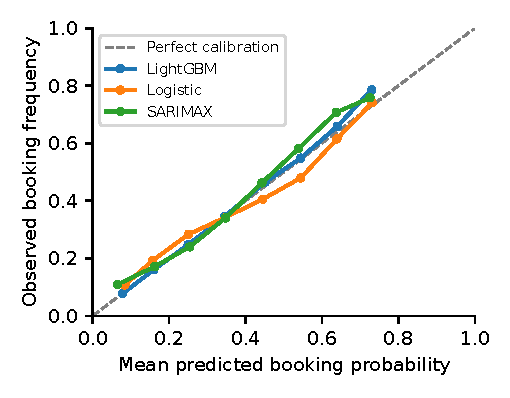
\includegraphics[width=\columnwidth]{reliability.pdf}
\caption{Test-set reliability on synthetic slots. Both axes are dimensionless probabilities. Points show ten equal-width probability bins with at least 20 observations; the dashed diagonal indicates equal predicted and observed booking rates.}
\label{fig:reliability}
\end{figure}


\begin{figure*}[t]
\centering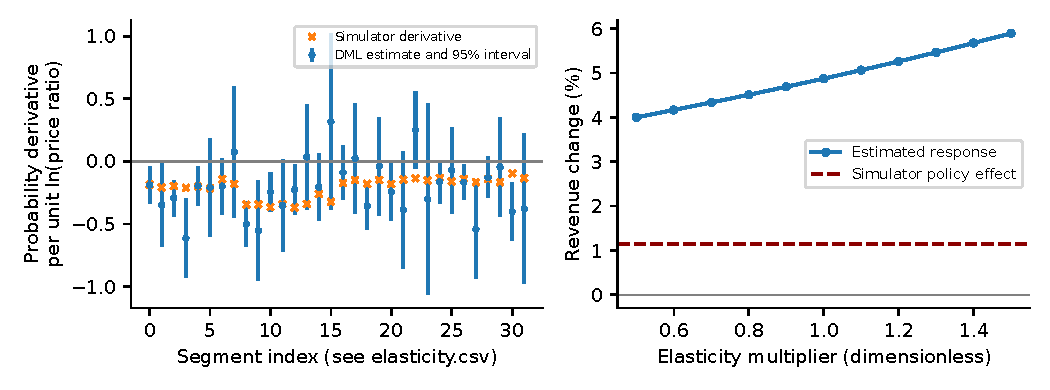
\includegraphics[width=.98\textwidth]{elasticity_sensitivity.pdf}
\caption{Price-response diagnostics on synthetic data. Left: estimated segment probability derivatives with 95\% clustered intervals and simulator average local derivatives; the segment index follows the saved elasticity table. Right: revenue change for the fixed chosen policy when estimated elasticities are multiplied by 0.5--1.5. The horizontal dashed line gives the known simulator effect for that policy.}
\label{fig:elasticity}
\end{figure*}


At the venue-day level, the LSTM had MAE 1.371 bookings per day and WAPE 28.05\%, compared with 1.378 and 28.19\% for LightGBM. Table~\ref{tab:secondary} gives the remaining values. These aggregated measures were not assessed with a separate paired test, so the reported ordering is descriptive. Aggregation changes the scored quantity from individual booking probabilities to the expected number of bookings across each venue-day.

\subsection{RQ2 Price response and counterfactual revenue}
Cross-fitting supplied 98,070 residual observations across 32 segments. Segment counts ranged from 531 to 7,195. The residual-to-observed log-price variance ratio ranged from 0.812 to 0.867, and all 32 segments met the sample-size and residual-variance thresholds. Five estimated probability derivatives were positive, although the simulator's local booking response to price was negative. Figure~\ref{fig:elasticity} shows the estimates and their intervals in the segment order retained in the accompanying CSV.

Against the simulator's average local derivative, the mean absolute discrepancy was 0.1647 for the orthogonalized estimate and 0.3125 for the naive estimate. The simulator derivative lay inside 29 of the 32 estimated intervals, or 90.6\%. This check compares the fitted partially linear coefficient with the average local derivative of the nonlinear generator. The two quantities have different statistical targets, so interval overlap is reported as a diagnostic.

The training revenue normalization factor was 1.0341. On test data, modeled revenue at historical prices divided by observed booking revenue was 0.9882. The corresponding modeled booking rate was 32.38\%, compared with the observed 32.58\%. The policy changed prices for 97.57\% of slots, and the mean recommended-to-historical price ratio was 1.0358. There were 20,259 price increases, 9,655 decreases and 746 unchanged prices, counting differences smaller than one millionth of a currency unit as unchanged. The no-change option remained available in the optimization. These recommendations were evaluated offline and were not implemented with customers. The demand diagnostics use the fitted price-response layer; checks using the generator's hidden booking probabilities are reported separately.

Table~\ref{tab:policy} reports a modeled revenue change of 4.87\%, with a 95\% interval of 3.28 to 6.79\%. Its lower bound exceeded the zero threshold, so the estimated-demand calculation satisfied H2. Evaluating exactly the same recommended prices under the simulator's known booking function gave 1.15\%. That value was below the lower endpoint of the estimated interval. The absolute difference between estimated and simulator revenue changes was 3.73 percentage points. No realized commercial revenue increase was observed.


\begin{table}[t]
\centering
\caption{Recommended minus historical policy on the same synthetic test slots. Estimated intervals combine venue-week resampling and 1,000 elasticity draws. The simulator column evaluates the fixed chosen prices using the known mechanism and is a deterministic expectation, not observed customer revenue.}
\label{tab:policy}
\footnotesize
\setlength{\tabcolsep}{3.5pt}
\begin{tabular}{lrrr}
\toprule
Outcome & Estimate & 95\% CI & Simulator \\
\midrule
Revenue change (\%) & 4.87 & [3.28, 6.79] & 1.15 \\
Utilization change (pp) & 0.56 & [0.02, 1.16] & -0.56 \\
Off-peak change (pp) & -0.31 & [-0.94, 0.33] & -0.92 \\
Cancellation change (pp) & -0.51 & [-0.69, -0.32] & -0.94 \\
\bottomrule
\end{tabular}
\end{table}

With the chosen policy held fixed, multiplying all estimated elasticities by a common factor from 0.5 to 1.5 produced revenue changes from 4.00\% to 5.90\%. Figure~\ref{fig:elasticity} shows the complete sensitivity curve. The calculated changes remained positive across the tested factors; no break-even factor was observed in this interval. The horizontal simulator value evaluates the same policy under its full known response, whereas the curve changes one shared multiplier in the estimated response model.

\subsection{RQ3 Off-peak occupancy and cancellations}
Under estimated demand, overall utilization changed by 0.56 percentage points, with an interval of 0.02 to 1.16. The simulator evaluation gave -0.56 percentage points for the same prices. The estimated response predicted an increase, while the simulator response gave a decrease in overall utilization. Off-peak occupancy changed by -0.31 percentage points under estimated demand, with an interval of -0.94 to 0.33; the corresponding simulator change was -0.92 percentage points.

The estimated cancellation-rate change was -0.51 percentage points, with an interval of -0.69 to -0.32. The training-derived non-inferiority margin was 0.75 percentage points, and the estimated upper bound was below that margin. The cancellation condition passed, but the lower bound for off-peak occupancy did not exceed zero. H3 was therefore not satisfied. Both cancellation rates use expected bookings as the denominator. Offered slots without a booking are excluded from that denominator.


\subsection{Additional analyses and observed errors}
Removing the four weather variables from every covariate step increased LightGBM's Brier score from 0.1951 to 0.1974 and log-loss from 0.5747 to 0.5806. The paired Brier difference was 0.0023, with a 95\% interval of 0.0017 to 0.0029. The corresponding log-loss interval was 0.0044 to 0.0073. The ablation was evaluated separately from the eight primary tests. Its bootstrap intervals are descriptive, and no multiplicity-adjusted significance is claimed for these additional comparisons.

Figure~\ref{fig:groups} compares observed and predicted booking rates by facility type. Football had an observed rate of 34.25\% and a predicted rate of 32.97\%, the largest absolute rate discrepancy among the four types. Swimming had the highest group Brier score, 0.2091; tennis had the lowest, 0.1845. Booking prevalence differs across these groups. The scores describe each group's prediction errors without establishing a controlled comparison of facility difficulty. The saved group table includes denominators, booked counts and log-loss for every type.

A further descriptive error check examined the 1,875 test slots with predicted booking probability of at least 0.60. Their mean prediction was 65.74\%, and 1,280 were booked, an observed rate of 68.27\%. The remaining 595 slots were unbooked despite receiving predictions above that threshold. The 0.60 threshold was used for this descriptive error check only. It had no role in model selection or recalibration.

The seasonal breakdown contains 11,340 spring slots and 19,320 summer slots. LightGBM's Brier score was 0.1793 in spring and 0.2043 in summer; the observed booking rates were 27.72\% and 35.43\%. No autumn or winter test scores were available. The test period therefore provides two seasonal groups, while all four seasons occur in the development data.

Several parts of the pipeline did not meet the specified checks. LightGBM's loss advantage over the LSTM was not supported, five estimated price derivatives were positive, and the simulator revenue effect fell outside the estimated interval. Estimated and simulator utilization changes also had opposite signs. H1 and H3 did not satisfy all their conditions. The selected model, price policy, test set and success thresholds were kept fixed after these outcomes were observed. Their causes and implications are left for the Discussion.


\begin{table}[t]
\centering
\caption{Venue-day errors after summing slot probabilities. MAE is measured in bookings per venue-day and WAPE is a percentage. These secondary measures use the same test slots as the main probability comparison.}
\label{tab:secondary}
\footnotesize
\setlength{\tabcolsep}{3.5pt}
\begin{tabular}{lrr}
\toprule
Model & MAE (bookings/day) & WAPE (\%) \\
\midrule
Climatology & 1.810 & 37.04 \\
Logistic & 1.677 & 34.32 \\
LightGBM & 1.378 & 28.19 \\
LSTM & 1.371 & 28.05 \\
SARIMAX & 1.400 & 28.64 \\
\bottomrule
\end{tabular}
\end{table}

\begin{figure}[t]
\centering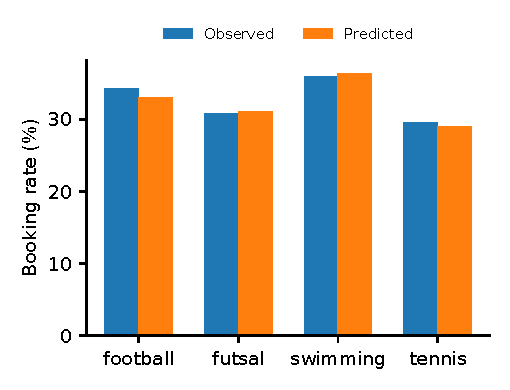
\includegraphics[width=\columnwidth]{group_errors.pdf}
\caption{Observed and LightGBM-predicted booking rates by synthetic facility type on the common test period. Football and futsal each have 8,760 slots; swimming and tennis each have 6,570. Bars show rates as percentages of offered slots.}
\label{fig:groups}
\end{figure}


\subsection{Reproducibility}
Repository publication is pending. The complete code, data, results and manuscript source accompany this article in the submission archive.

The run used Python 3.12.14, NumPy 2.3.5, pandas 2.2.3, scikit-learn 1.8.0, SciPy 1.17.0, LightGBM 4.7.0, Optuna 5.0.0, PyTorch 2.14.1{+}cpu and statsmodels 0.15.0. The execution platform was Linux on an AMD EPYC 9V74 80-Core Processor, with 9 logical CPUs visible and two computation threads configured for the fitted models. No GPU was used. A clean analysis run took approximately 6.0 minutes in this environment, excluding package installation and manuscript compilation; runtime on another computer will differ.

The generator and tuning seeds were 2026, model seeds were 0--4, the forecast bootstrap seed was 2026, and the combined elasticity and policy bootstrap used seed 123. The package records split boundaries, search trials, selected hyperparameters, per-seed scores, test predictions, paired tests, elasticity estimates and simulator checks. It includes a script that checks reported scores against saved predictions and verifies the test membership, temporal gaps, price grid and revenue arithmetic. All tabular values and vector figures in this section can be regenerated from the supplied data and code.
\FloatBarrier

\balance
\bibliographystyle{IEEEtran}
\bibliography{references}
\end{document}
